\documentclass[tikz,border=6pt]{standalone}
\usepackage{amsmath}
\usetikzlibrary{arrows.meta,positioning}
\usepackage[dvipsnames]{xcolor}

\begin{document}
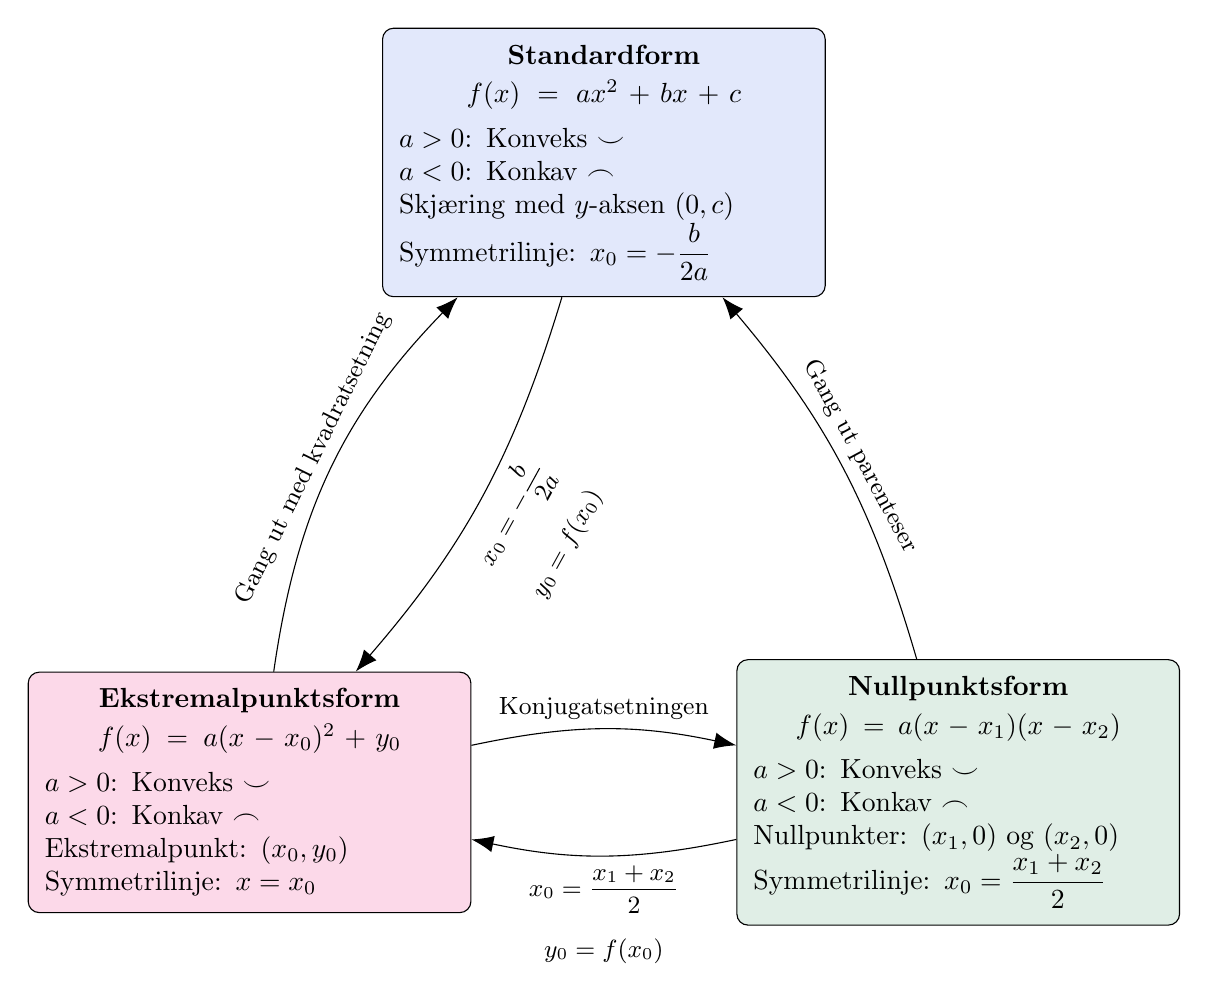
\begin{tikzpicture}[
  >={Latex[length=2.8mm]},
  box/.style   = {
    draw, rounded corners,
    align=center,
    inner sep=6pt,
    minimum width=\boxw,
    text width=\boxw,   % prevent width from growing
    fill=black!3
  },
  label/.style = {font=\small, align=center}
]

% ---- constants ----
\def\L{9}            % triangle side length
\def\H{8}          % height ~ (sqrt3/2)*L
\def\boxw{52mm}       % fixed width for every box

% ---- nodes (equilateral triangle) ----
\node[box, fill=RoyalBlue!15] (std) at (0,\H) {
  \textbf{Standardform}\\[2pt]
  $f(x)=ax^2+bx+c$\\[4pt]
  % selectively left-align these two lines:
  \makebox[\boxw][l]{\normalsize $a > 0$: Konveks $\smile$}\\
  \makebox[\boxw][l]{\normalsize $a < 0$: Konkav $\frown$}\\
  \makebox[\boxw][l]{\normalsize Skjæring med $y$-aksen $(0, c)$}\\
  \makebox[\boxw][l]{\normalsize Symmetrilinje: $x_0=-\dfrac{b}{2a}$}
};

\node[box, fill=RubineRed!15] (ext) at (-\L/2,0) {
  \textbf{Ekstremalpunktsform}\\[2pt]
  $f(x)=a(x-x_0)^2+y_0$\\[4pt]
  \makebox[\boxw][l]{\normalsize $a > 0$: Konveks $\smile$}\\
  \makebox[\boxw][l]{\normalsize $a < 0$: Konkav $\frown$} \\
  \makebox[\boxw][l]{\normalsize Ekstremalpunkt: $(x_0, y_0)$}\\
  \makebox[\boxw][l]{\normalsize Symmetrilinje: $x = x_0$}\\
};

\node[box, fill=SeaGreen!15] (nul) at (\L/2,0) {
  \textbf{Nullpunktsform}\\[2pt]
  $f(x)=a(x-x_1)(x-x_2)$\\[4pt]
  \makebox[\boxw][l]{\normalsize $a > 0$: Konveks $\smile$}\\
  \makebox[\boxw][l]{\normalsize $a < 0$: Konkav $\frown$} \\
  \makebox[\boxw][l]{\normalsize Nullpunkter: $(x_1, 0)$ og $(x_2, 0)$}\\
  \makebox[\boxw][l]{\normalsize Symmetrilinje: $x_0 = \dfrac{x_1 + x_2}{2}$}\\
};

% ---- arrows (circular-style bends) ----
\draw[->] (std) to[bend left=12]
  node[label,midway,sloped,below] {$x_0=-\dfrac{b}{2a}$\\ \\ $y_0=f(x_0)$}
  (ext);

\draw[->] (ext) to[bend left=12]
  node[label,midway,sloped,above] {Konjugatsetningen}
  (nul);

\draw[->] (nul) to[bend left=12]
  node[label,midway,sloped,below] {$x_0=\dfrac{x_1+x_2}{2}$\\ \\ $y_0=f(x_0)$}
  (ext);

\draw[->] (nul) to[bend right=12]
  node[label,midway,sloped,above] {Gang ut parenteser}
  (std);

\draw[->] (ext) to[bend left=18]
  node[label,midway,sloped,above] {Gang ut med kvadratsetning}
  (std);

\end{tikzpicture}
\end{document}